\documentclass[DaoFP]{subfiles}
\begin{document}
\setcounter{chapter}{9}

\chapter{Adjunctions}

A sculptor subtracts irrelevant stone until a sculpture emerges. A mathematician abstracts irrelevant details until a pattern emerges.

We were able to define a lot of constructions using their mapping-in and mapping-out properties. Those, in turn, could be compactly written as isomorphisms between hom-sets. This pattern of natural isomorphisms between hom-sets is called an adjunction and, once recognized, pops up virtually everywhere.

\section{The Currying Adjunction}

The definition of the exponential is the classic example of an adjunction that relates mappings-out and mappings-in. Every mapping out of a product corresponds to a unique mapping into the exponential:
\[  \mathcal{C}(e \times a, b ) \cong  \mathcal{C} (e, b^a)  \]
The object $b$ takes the role of the focus on the left hand side; the object $e$ becomes the observer on the right hand side. 

We can spot two functors at play. They are both parameterized by $a$. On the left we have the product functor $(- \times a)$ applied to $e$. On the right we have the exponential functor $(-)^a$ applied to $b$. 

If we write these functors as:
\[ L_a e = e \times a \]
\[ R_a b = b^a \]
then the natural isomorphism
\[ \mathcal{C}(L_a e, b) \cong \mathcal{C}(e, R_a b) \]
is called the adjunction between them. 

In components, this isomorphism tells us that, given a mapping $\phi \in \mathcal{C}(L_a e, b)$, there is a unique mapping $\phi^T \in \mathcal{C}(e, R_a b)$ and vice versa. These mappings are sometimes called the \emph{transpose} of each other---the nomenclature taken from matrix algebra.

The shorthand notation for the adjunction is $L \dashv R$. Substituting the product functor for $L$ and the exponential functor for $R$, we can write the currying adjunction concisely as:

\[ (- \times a) \dashv (-)^a \]

The exponential object $b^a$ is sometimes called the \index{internal hom}\emph{internal hom} and is written as $[a, b]$. This is in contrast to the \emph{external hom}, which is the set $\cat C (a, b)$. The external hom is \emph{not} an object in $\cat C$ (except when $\cat C$ itself is $\Set$). With this notation, the currying adjunction can be written as:
\[  \mathcal{C}(e \times a, b) \cong  \mathcal{C} (e, [a, b])  \]
A category in which this adjunction holds is called cartesian closed.

Since functions play central role in every programming language, cartesian closed categories form the basis of all models of programming. We interpret the exponential $b^a$ as the function type $a \to b$. 

Here $e$ plays the role of the external environment---the $\Gamma$ of the lambda calculus. The morphism in $\cat C(\Gamma \times a, b)$ is interpreted as an expression of type $b$ in the environment $\Gamma$ extended by a variable of type $a$. The function type $a \to b$ therefore represents a closure that may capture a value of type $e$ from its environment.

Incidentally, the category of (small) categories $\mathbf{Cat}$ is also cartesian closed, as reflected in this adjunction between product categories and functor categories that uses the same internal-hom notation:
\[ \mathbf{Cat} (\cat A \times \cat B, \cat C) \cong \mathbf{Cat} (\cat A, [\cat B, \cat C]) \]
Here, both sides are sets of natural transformations.


\section{The Sum and the Product Adjunctions}

The currying adjunction relates two endofunctors, but an adjunction can be easily generalized to functors that go between different categories. Let's see some examples first.

\subsection{The diagonal functor}

The sum and the product types were defined using bijections where one of the sides was a single arrow and the other was a pair of arrows. A pair of arrows can be seen as a single arrow in the product category. 

To explore this idea, we need to define the diagonal functor $\Delta$, which is a special mapping from $\mathcal{C}$ to $\mathcal{C} \times \mathcal{C}$. It takes an object $x$ and duplicates it, producing a pair of objects $\langle x, x \rangle$. It also takes an arrow $f$ and duplicates it $\langle f, f \rangle$.

Interestingly, the diagonal functor is related to the constant functor we've seen previously. The constant functor can be though of as a functor of two variables---it just ignores the second one. We've seen this in the Haskell definition:
\begin{haskell}
data Const c a = Const c
\end{haskell}

To see the connection, let's look at the product category $\mathcal{C} \times \mathcal{C}$ as a functor category $[ \mathbf{2}, \mathcal{C}]$, in other words, the exponential object $\mathcal{C}^{ \mathbf{2}}$ in $\mathbf{Cat}$. Indeed, a functor from $\mathbf{2}$ (the stick-figure category with two objects) picks a pair of objects---which is equivalent to a single object in the product category.


A functor $\mathcal{C} \to [\mathbf{2}, \mathcal{C}]$ can be uncurried to $\mathcal{C} \times \mathbf{2} \to  \mathcal{C}$. The diagonal functor ignores the second argument, the one coming from $\mathbf{2}$: it does the same thing whether the second argument is $1$ or $2$. That's exactly what the constant functor does as well. This is why we use the same symbol $\Delta$ for both.

Incidentally, this argument can be easily generalized to any indexing category, not just $\mathbf{2}$.

\subsection{The sum adjunction}

Recall that the sum is defined by its mapping out property. There is a one-to one correspondence between the arrows coming out of the sum $a + b$ and pairs of arrows coming from $a$ and $b$ separately. In terms of hom-sets, we can write it as:
\[  \mathcal{C} (a + b, x) \cong \mathcal{C}( a , x) \times \mathcal{C}( b , x)\]
where the product on the right-hand side is just a cartesian product of sets, that is the set of pairs. Moreover, we've seen earlier that this bijection is natural in $x$.

We know that a pair of arrows is a single arrow in the product category. We can, therefore, look at the elements on the right-hand side as arrows in $\mathcal{C} \times \mathcal{C}$ going from the object $\langle a, b \rangle$ to the object $\langle x, x \rangle$. The latter can be obtained by acting with the diagonal functor $\Delta$ on $x$. We have:

\[  \mathcal{C} (a + b, x) \cong (\mathcal{C} \times \mathcal{C})( \langle a, b \rangle , \Delta x)\]
This is a bijection between hom-sets in two different categories. It satisfies naturality conditions, so it's a natural isomorphism. 

We can spot a pair of functors here as well. On the left we have the functor that takes a pair of objects $\langle a, b \rangle$ and produces their sum $a + b$:
\[ (+) \colon \mathcal{C} \times \mathcal{C} \to \mathcal{C}\]
On the right-hand side, we have the diagonal functor $\Delta$ going in the opposite direction:
\[ \Delta \colon \mathcal{C} \to  \mathcal{C} \times \mathcal{C} \]
Altogether, we have a pair of functors between a pair of categories:
\[
 \begin{tikzcd}
  \mathcal{C}
   \arrow[rr, bend right, "\Delta"']
  &&
  \mathcal{C} \times \mathcal{C}
 \arrow[ll, bend right, "(+)"']
  \end{tikzcd}
\]
and an isomorphism between the hom-sets:
\[
 \begin{tikzcd}
a + b
\arrow[d, bend right, red, dashed]
\arrow[d, dashed]
\arrow[d, bend left, blue, dashed]
  &&
 \langle a , b \rangle
\arrow[d, bend right, red, dashed]
\arrow[d, dashed]
\arrow[d, bend left, blue, dashed]
 \arrow[ll, bend right, "(+)"']
 \\
 x
   \arrow[rr, bend right, "\Delta"']
 &&
 \langle x, x \rangle
  \end{tikzcd}
\]
In other words, we have the adjunction:
\[ (+) \dashv \Delta \]


\subsection{The product adjunction}

We can apply the same reasoning to the definition of a product. This time we have a natural isomorphism between pairs of arrows and a mapping \emph{into} the product.

\[  \mathcal{C} (x, a) \times \mathcal{C}(x, b) \cong  \mathcal{C} (x, a \times b)  \]
Replacing pairs of arrows with arrows in the product category we get:

\[  (\mathcal{C} \times \mathcal{C})( \Delta x,  \langle a, b \rangle ) \cong  \mathcal{C} (x, a \times b)  \]
These are the two functors going in the opposite direction:
\[
 \begin{tikzcd}
  \mathcal{C} \times \mathcal{C}
  \arrow[rr, bend right, "(\times)"']
  &&
  \mathcal{C}
  \arrow[ll, bend right, "\Delta"']
  \end{tikzcd}
\]
and this is the isomorphism of hom-sets:

\[
 \begin{tikzcd}
 \langle x, x \rangle
\arrow[d, bend right, red, dashed]
\arrow[d, dashed]
\arrow[d, bend left, blue, dashed]
  &&
  x
\arrow[d, bend right, red, dashed]
\arrow[d, dashed]
\arrow[d, bend left, blue, dashed]
 \arrow[ll, bend right, "\Delta"']
 \\
 \langle a , b \rangle
   \arrow[rr, bend right, "(\times)"']
 &&
 a \times b
  \end{tikzcd}
\]
In other words, we have the adjunction:
\[ \Delta \dashv (\times) \]

\subsection{Distributivity}

In a bicartesian closed category products distribute over sums. We've seen one direction of the proof using universal constructions. Adjunctions combined with the Yoneda lemma give us more powerful tools to tackle this problem.

We want to show the natural isomorphism:
\[(b + c) \times a \cong b \times a + c \times a \]
Instead of proving this identity directly, we'll show that the mappings out from both sides to an arbitrary object $x$ are isomorphic:
\[  \mathcal{C} ((b + c) \times a, x) \cong \mathcal{C}(b \times a + c \times a, x) \]
The left hand side is a mapping out of a product, so we can apply the currying adjunction to it:
\[  \mathcal{C} ((b + c) \times a, x) \cong \mathcal{C}(b + c, x^a) \]
This gives us a mapping out of a sum which, by the sum adjunction is isomorphic to the product of two mappings:
\[  \mathcal{C}(b + c, x^a) \cong \mathcal{C}(b, x^a) \times \mathcal{C}(c, x^a)\]
We can now apply the inverse of the currying adjunction to both components:
\[  \mathcal{C}(b, x^a) \times \mathcal{C}(c, x^a) \cong \mathcal{C}(b \times a, x) \times \mathcal{C}(c \times a, x)\]
Using the inverse of the sum adjunction, we arrive at the final result:
\[ \mathcal{C}(b \times a, x) \times \mathcal{C}(c \times a, x) \cong \mathcal{C}(b \times a + c \times a, x) \]

Every step in this proof was a natural isomorphism, so their composition is also a natural isomorphism. By Yoneda lemma, the two objects that form the left- and the right-hand side of distributivity law are therefore isomorphic.

A much shorter proof of this statement follows from the property of left adjoints that we'll discuss soon.

\section{Adjunction between functors}

In general, an adjunction relates two functors going in opposite directions between two categories. The left functor 
\[ L \colon \mathcal{D} \to \mathcal{C}\]
and the right functor:
\[ R \colon \mathcal{C} \to  \mathcal{D} \]
The adjunction $L \dashv R$ is defined as a natural isomorphism between two hom-sets.
\[  \mathcal{C} (L x, y) \cong \mathcal{D}( x , R y)\]
In other words, we have a family of invertible functions between sets:
\[ \phi_{x y} \colon  \mathcal{C} (L x, y) \to \mathcal{D}( x , R y) \]
natural in both $x$ and $y$. For instance, naturality in $y$ means that, for any $f \colon y \to y'$ the following diagram commutes:
\[
 \begin{tikzcd}
 \mathcal{C}(L x, y)
 \arrow[d, leftrightarrow, "\phi_{x y}"]
 \arrow[r, "{\mathcal{C}(L x, f)}"]
 &
 \mathcal{C}(L x, y')
  \arrow[d, leftrightarrow, "\phi_{x y'}"]
 \\
 \mathcal{D}(x, R y)
 \arrow[r, "{\mathcal{D}(x, R f)}"]
& \mathcal{D}(x, R y')
 \end{tikzcd}
\]
or, considering that a lifting of arrows by hom-functors is the same as post-composition:
\[
 \begin{tikzcd}
 \mathcal{C}(L x, y)
 \arrow[d, leftrightarrow, "\phi_{x y}"]
 \arrow[r, "f \circ -"]
 &
 \mathcal{C}(L x, y')
  \arrow[d, leftrightarrow, "\phi_{x y'}"]
 \\
 \mathcal{D}(x, R y)
 \arrow[r, "R f \circ -"]
& \mathcal{D}(x, R y')
 \end{tikzcd}
\]
The double-headed arrows can be traversed in either direction (using $\phi^{-1}_{x y}$ when going up), since they are the components of an isomorphism.


Pictorially, we have two functors:
\[
 \begin{tikzcd}
  \mathcal{C}
  \arrow[rr, bend right, "R"']
  &&
  \mathcal{D}
  \arrow[ll, bend right, "L"']
  \end{tikzcd}
\]
and, for any pair $x$ and $y$, two isomorphic hom-sets:
\[
 \begin{tikzcd}
L x
\arrow[d, bend right, red, dashed]
\arrow[d, dashed]
\arrow[d, bend left, blue, dashed]
  &&
  x
\arrow[d, bend right, red, dashed]
\arrow[d, dashed]
\arrow[d, bend left, blue, dashed]
 \arrow[ll, bend right, "L"']
 \\
y
   \arrow[rr, bend right, "R"']
 &&
 R y
  \end{tikzcd}
\]
 These hom-sets come from two different categories, but sets are just sets. We say that $L$ is the left adjoint of $R$, or that $R$ is the right adjoint of $L$

In Haskell, the simplified version of this could be encoded as a multi-parameter type class:
\begin{haskell}
class (Functor left, Functor right) => Adjunction left right where
  ltor :: (left x -> y) -> (x -> right y)
  rtol :: (x -> right y) -> (left x -> y)
\end{haskell}
It requires the following pragma at the top of the file:
\begin{haskell}
{-# language MultiParamTypeClasses #-}
\end{haskell}



Therefore, in a bicartesian category, the sum is the left adjoint to the diagonal functor; and the product is its right adjoint. We can write this very concisely (or we could impress it in clay, in a modern version of cuneiform):
\[ (+) \dashv \Delta \dashv (\times) \]

\begin{exercise}
Draw the commuting square witnessing the naturality of the adjunction function $\phi_{x y}$ in $x$.
\end{exercise}

\begin{exercise}
The hom-set $\mathcal{C} (L x, y)$ on the left-hand side of the adjunction formula suggests that $L x$ could be seen as a representing object for some functor (a co-presheaf). What is this functor? Hint: It maps $y$ to a set. What set is it?
\end{exercise}

\begin{exercise}
Conversely, a representing object $a$ for a presheaf $P$ is defined by:
\[P x \cong \mathcal{D}(x, a)\]
What is the presheaf for which $R y$, in the adjunction formula, is the representing object.
\end{exercise}

\section{Limits and Colimits as Adjunctions}

The definition of a limit also involves a natural isomorphism between hom-sets:
\[ [\cat J, \mathcal{C}](\Delta_x, D)  \cong \mathcal{C}(x, \text{Lim} D) \]
The hom-set on the left is in the functor category. Its elements are cones, or natural transformations between the constant functor $\Delta_x$ and the diagram functor $D$. The one on the right is a hom-set in $\mathcal{C}$. 

In a category where all limits exist, we have the adjunction between these two functors:
\[ \Delta_{(-)} \colon \mathcal{C} \to  [\cat J, \mathcal{C}] \]
and:
\[ \text{Lim}{(-)} \colon  [\cat J, \mathcal{C}] \to \mathcal{C} \]

Dually, the colimit is described by the following natural isomorphism:
\[ [\cat J, \mathcal{C}](D, \Delta_x)  \cong \mathcal{C}( \text{Colim} D, x) \]
We can write both adjunctions using one terse formula:
\[ \text{Colim} \dashv \Delta \dashv \text{Lim}\]

In particular, since the product category $\cat C \times \cat C$ is equivalent to $\cat C^2$, or the functor category $[\mathbf{2}, \cat C]$, we can rewrite a product and a coproduct as a limit and a colimit:
\[ [\mathbf{2}, \cat C](\Delta_x, \langle a, b \rangle) \cong \cat C(x, a \times b) \]
\[ \cat C( a + b, x) \cong [\mathbf{2}, \cat C]( \langle a, b \rangle, \Delta_x) \]
where $\langle a, b \rangle$ denotes a diagram that is the action of a functor $D \colon \mathbf{2} \to \cat C$ on the two objects of $\mathbf{2}$.

\section{Unit and Counit of an Adjunction}

We compare arrows for equality, but we prefer to use isomorphisms for comparing objects. 

We have a problem when it comes to functors, though. On the one hand, they are objects in the functor category, so isomorphisms are the way to go; on the other hand, they are arrows in $\mathbf{Cat}$ so maybe it's okay to compare them for equality?

To shed some light on this dilemma, we should ask ourselves \emph{why} we use equality for arrows. It's not because we like equality, but because there's nothing else for us to do in a set but to compare elements for equality. Two elements of a hom-set are either equal or not, period. 

That's not the case in  $\mathbf{Cat}$ which, as we know, is a $2$-category. Here, hom-sets themselves have the structure of a category---the functor category. In a $2$-category we have arrows between arrows so, in particular, we can define isomorphisms between arrows. In $\mathbf{Cat}$ these would be natural isomorphisms between functors.

However, even though we have the option of replacing arrow equalities with isomorphisms, categorical laws in $\mathbf{Cat}$ are still expressed as equalities. For instance, the composition of a functor $F$ with the identity functor is \emph{equal} to $F$, and the same for associativity. A $2$-category in which the laws are satisfied ``on the nose'' is called \emph{strict}, and $\mathbf{Cat}$ is an example of a strict $2$-category. 

But as far as comparing categories goes, we have more options. Categories are objects in $\mathbf{Cat}$, so it's possible to define an isomorphism of categories as a pair of functors $L$ and $R$:
\[
 \begin{tikzcd}
  \mathcal{C}
  \arrow[rr, bend right, "R"']
  \arrow[loop, "\text{Id}_{ \mathcal{C}} "']
  &&
  \mathcal{D}
  \arrow[ll, bend right, "L"']
  \arrow[loop, "\text{Id}_{ \mathcal{D}} "']
  \end{tikzcd}
\]
such that:
\begin{align*}
L \circ R = \text{Id}_{ \mathcal{C}} \\
\text{Id}_{ \mathcal{D}} = R \circ L 
\end{align*}
This definition involves equality of functors, though. What's worse, acting on objects, it involves equality of objects:
\begin{align*}
 L (R x) = x \\
 y = R (L y)
\end{align*}
This is why it's more proper to talk about a weaker notion of \emph{equivalence} of categories, where equalities are replaced by isomorphisms:
\begin{align*}
L \circ R \cong \text{Id}_{ \mathcal{C}} \\
 \text{Id}_{ \mathcal{D}} \cong R \circ L 
\end{align*}
On objects, an equivalence of categories means that a round trip produces an object that is isomorphic, rather than equal, to the original one. In most cases, this is exactly what we want.

An adjunction is also defined as a pair of functors going in opposite directions, so it makes sense to ask what the result of a round trip is. 

The isomorphism that defines an adjunction works for any pair of objects $x$ and $y$
\[  \mathcal{C} (L x, y) \cong \mathcal{D}( x , R y)\]
so, in particular, it works if we replace $y$ with $L x$
\[  \mathcal{C} (L x, L x) \cong \mathcal{D}( x , R (L x))\]
We can now use the Yoneda trick and pick the identity arrow $id_{L x}$ on the left. The isomorphism maps it to a unique arrow on the right, which we'll call $\eta_x$:
\[ \eta_x \colon x \to R ( L x) \]
Not only is this mapping defined for every $x$, but it's also natural in $x$. The natural transformation $\eta$ is called the \emph{unit} of the adjunction. If we observe that the $x$ on the left is the action of the identity functor on $x$, we can write:
\[ \eta \colon \text{Id}_{\mathcal{D}} \to R \circ L \]

As an example, let's evaluate the unit of the coproduct adjunction:
\[  \mathcal{C} (a + b, x) \cong (\mathcal{C} \times \mathcal{C})( \langle a, b \rangle , \Delta x)\]
by replacing $x$ with $a + b$. We get:
\[ \eta_{\langle a, b \rangle} \colon \langle a, b \rangle \to \Delta(a + b) \]
This is a pair of arrows that are exactly the two injections $\langle \text{Left}, \text{Right} \rangle$.

We can do a similar trick by replacing $x$ with $R y$:
\[  \mathcal{C} (L (R y), y) \cong \mathcal{D}( R y , R y)\]
Corresponding to $id_{R y}$ on the right, we get an arrow on the left:
\[ \varepsilon_y \colon L (R y) \to y \]
These arrows form another natural transformation called the \emph{counit} of the adjunction:
\[ \varepsilon \colon L \circ R \to \text{Id}_{\mathcal{C}}  \]

Notice that, if those two natural transformations were invertible, they would witness the equivalence of categories. But even if they're not, this kind of ``half-equivalence'' is still very interesting in the context of category theory. 

As an example, let's evaluate the counit of the product adjunction:
\[  (\mathcal{C} \times \mathcal{C})( \Delta x,  \langle a, b \rangle ) \cong  \mathcal{C} (x, a \times b)  \]
by replacing $x$ with $a \times b$. We get:
\[ \varepsilon_{\langle a, b \rangle} \colon \Delta (a \times b) \to \langle a, b \rangle \]
This is a pair of arrows that are exactly the two projections $\langle \text{fst}, \text{snd} \rangle$.

\begin{exercise}
Derive the counit of the coproduct adjunction and the unit of the product adjunction.
\end{exercise}

\subsection{Triangle identities}

We can use the unit/counit pair to formulate an equivalent  definition of an adjunction. To do that, we start with a pair of natural transformations:
\begin{align*}
\eta \colon \text{Id}_{\mathcal{D}} \to R \circ L \\
\varepsilon \colon L \circ R \to \text{Id}_{\mathcal{C}} 
\end{align*}
and impose additional \emph{triangle identities}. 

These identities can be derived from the standard definition of the adjunction by noticing that $\eta$ can be used to replace an identity functor with the composite $R \circ L$, effectively letting us insert $R \circ L$ anywhere an identity functor would work.

Similarly, $\varepsilon$ can be used to eliminate the composite $L \circ R$ (i.e., replace it with identity). 

So, for instance, starting with $L$:
\[ L = L \circ \text{Id}_{\mathcal{D}} \xrightarrow{L \circ \eta} L \circ R \circ L \xrightarrow{\varepsilon \circ L} \text{Id}_{\mathcal{C}} \circ L = L \]
Here, we used the horizontal composition of natural transformation, with one of them being the identity transformation (a.k.a., whiskering).

The first triangle identity is the condition that this chain of transformations result in the identity natural transformation. Pictorially:

\[
 \begin{tikzcd}
 L
 \arrow[r, "L \circ \eta"]
 \arrow[rd, "id_L"']
 & L \circ R \circ L
 \arrow[d, "\varepsilon \circ L"]
 \\
 & L
  \end{tikzcd}
\]

Similarly, we want the following chain of natural transformations to also compose to identity:
\[ R = \text{Id}_{\mathcal{D}} \circ R \xrightarrow{\eta \circ R} R \circ L \circ R \xrightarrow{R \circ \varepsilon} R \circ \text{Id}_{\mathcal{C}} = R \]
or, pictorially:
\[
 \begin{tikzcd}
 R
 \arrow[r, "\eta \circ R"]
 \arrow[rd, "id_R"']
 & R \circ L \circ R
 \arrow[d, "R \circ \varepsilon"]
 \\
 & R
  \end{tikzcd}
\]

It turns out that an adjunction can be alternatively defined in terms of the two natural transformations, $\eta$ and $\varepsilon$, satisfying the  triangle identities:
\begin{align*}
(\varepsilon \circ L) \cdot (L \circ \eta) = id_L \\
(R \circ \varepsilon) \cdot (\eta \circ R) = id_R
\end{align*}

From those, the mapping of hom-sets can be easily recovered. For instance, let's start with an arrow $f \colon x \to R y$, which is an element of $\mathcal{D}( x , R y)$. We can lift it to 
\[L f \colon L x \to L (R y)\]
We can then use $\eta$ to collapse the composite $L \circ R$ to identity. The result is an arrow $L x \to y$, which is an element of $ \mathcal{C} (L x, y)$.


The definition of the adjunction using unit and counit is more general in the sense that it can be translated to an arbitrary 2-category setting. 

\begin{exercise}
Given an arrow $g \colon L x \to y$ implement an arrow $x \to R y$ using $\varepsilon$ and the fact that $R$ is a functor. Hint: Start with the object $x$ and see how you can get from there to $R y$ with one stopover.
\end{exercise}

\subsection{The unit and counit of the currying adjunction}

Let's calculate the unit and the counit of the currying adjunction:
\[  \mathcal{C}(e \times a, b ) \cong  \mathcal{C} (e, b^a)  \]
If we replace $b$ with $e \times a$, we get
\[  \mathcal{C}(e \times a, e \times a ) \cong  \mathcal{C} (e, (e \times a)^a)  \]
Corresponding to the identity arrow on the left, we get the unit of the adjunction on the right:
\[ \eta \colon e \to (e \times a)^a \]
This is a curried version of the product constructor. In Haskell, we write it as:
\begin{haskell}
unit :: e -> (a -> (e, a))
unit = curry id
\end{haskell}

The counit is more interesting. Replacing $e$ with $b^a$ we get:
\[  \mathcal{C}(b^a \times a, b ) \cong  \mathcal{C} (b^a, b^a)  \]
Corresponding to the identity arrow on the right, we get:
\[ \varepsilon \colon b^a \times a \to b \]
which is the function application arrow. 

In Haskell:
\begin{haskell}
counit :: (a -> b, a) -> b
counit = uncurry id
\end{haskell}

When the adjunction is between two endofunctors, we can write an alternative Haskell definition of it using the unit and the counit:
\begin{haskell}
class (Functor left, Functor right) => 
  Adjunction left right | left -> right, right -> left where
    unit   :: x -> right (left x)
    counit :: left (right x) -> x
\end{haskell}
The additional two clauses \hask{left -> right} and \hask{right -> left} tell the compiler that, when using an instance of the adjunction, one functor can be derived from the other. This definition requires the following compile extensions:
\begin{haskell}
{-# language MultiParamTypeClasses #-}
{-# LANGUAGE FunctionalDependencies #-}
\end{haskell}

The two functors that form the currying adjunction can be written as:
\begin{haskell}
data L r x = L (x, r)    deriving (Functor, Show)
data R r x = R (r -> x)  deriving Functor
\end{haskell}
and the \hask{Adjunction} instance for currying is:
\begin{haskell}
instance Adjunction (L r) (R r) where
  unit x = R (\r -> L (x, r)) 
  counit (L (R f, r)) = f r
\end{haskell}
The first triangle identity states that the following polymorphic function:
\begin{haskell}
triangle :: L r x -> L r x
triangle = counit . fmap unit
\end{haskell}
is the identity, and so is the second one: 
\begin{haskell}
triangle' :: R r x -> R r x
triangle' = fmap counit . unit
\end{haskell}
Notice that these two functions require the use of functional dependencies to be well defined. Triangle identities cannot be expressed in Haskell, so it's up to the implementor of the adjunction to prove them.
\begin{exercise}
Test a few examples of the first triangle identity for the currying adjunction. Here's an example:
\begin{haskell}
triangle (L (2, 'a'))
\end{haskell}
\end{exercise}

\begin{exercise}
How would you test the second triangle identity for the currying adjunction? Hint: the result of \hask{triangle'} is a function, so you can't display it, but you could call it.
\end{exercise}

\section{Adjunctions Using Universal Arrows}

We've seen the definition of an adjunction using the isomorphism of hom-sets, and another one using the pair of unit/counit. It turns out that we can define an adjunction using just one element of this pair, as long as it satisfies certain universality condition. To see that, we will construct a new category whose objects are arrows. 

We've seen before an example of such a category---the slice category $\cat C/ c$ that collects all the arrows that converge on $c$. Such a category describes the view of the object $c$ from every possible angle in $\cat C$. 

\subsection{Comma category}
When dealing with an adjunction:
\[  \mathcal{C} (L d, c) \cong \mathcal{D}( d , R c)\]
we are observing the object $c$ from a narrower perspective defined by the functor $L$. Think of $L$ as defining a model of the category $\cat D$ inside $\cat C$. We are interested in the view of $c$ from the perspective of this model. The arrows that describe this view form the comma category $L/c$.


\[
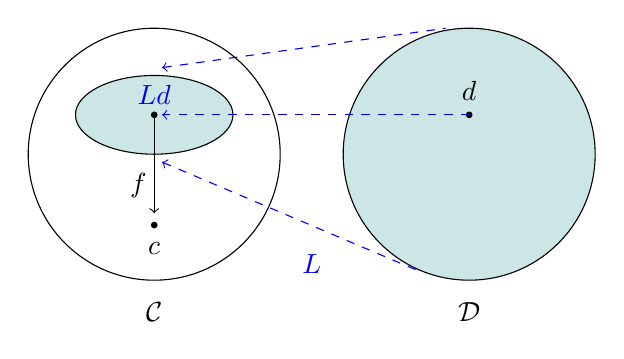
\begin{tikzpicture}
  \def\Xa{2.0};
  \def\Xb{-2.0};
  
  \def\Ytip{-0.9};
  \def\Yo{0.5}; % oval
  \def\Yb{-2.0}; % labels
         \draw (\Xa, 0)[fill=blue!50!green!20]  ellipse (1.6 and 1.6);
         \draw (\Xb , 0) ellipse (1.6 and 1.6);
         % oval
         \draw (\Xb , \Yo)[fill=blue!50!green!20] ellipse (1 and 0.5);
         
        % apex
        \filldraw (\Xb, \Ytip) circle (1pt);
        \node at ( \Xb, \Ytip - 0.3) { $c$ };
        
        % image
        \filldraw (\Xa, \Yo) circle (1pt);
        \node at ( \Xa, \Yo + 0.3) { $d$ };
        
	% middle of the cone
	\draw[->] (\Xb, \Yo) -- (\Xb, \Ytip + 0.15);
	\node at (\Xb - 0.2, \Ytip + 0.5) {$f$};
        	% sides of the cone
	%\draw (\Xb, \Ytip) -- (\Xb + 0.95, \Yo - 0.15);
	%\draw (\Xb, \Ytip) -- (\Xb - 0.95, \Yo - 0.15);

        % categories
        \node at (\Xa, \Yb) { $\mathcal D$ };
        \node at (\Xb, \Yb) { $\mathcal C$ };
        \node[blue] at (0, \Yb + 0.6) { $L$ };

        % functor middle
        \filldraw (\Xb, \Yo) circle (1pt);
        \node[blue] at ( \Xb, \Yo + 0.25) { $L d$ };
	\draw[->, blue, dashed] (\Xa, \Yo) -- (\Xb + 0.1, \Yo);
	% functor 
	\draw [<-, blue, dashed] (\Xb + 0.1, \Yo + 0.6)   --   (\Xa - 0.3, \Yo + 1.1);
	\draw [<-,blue, dashed] (\Xb + 0.1, \Yo - 0.6) -- (\Xa - 0.6, \Ytip - 0.6);
\end{tikzpicture}
\]



An object in the \index{comma category}\emph{comma category} $L/c$ is a pair $\langle d, f \rangle$, where $d$ is an object of $\cat D$ and $f \colon L d \to c$ is an arrow in $\cat C$. 

A morphism from $\langle d, f \rangle$ to $\langle d', f' \rangle$ is an arrow $h \colon d \to d'$ that makes the diagram on the left commute:
\[
 \begin{tikzcd}
 L d
 \arrow[rd, "f"']
 \arrow[rr, "L h"]
 && L d'
 \arrow[ld, "f'"]
 \\
 &c
  \end{tikzcd}
 \hspace{30pt}
\begin{tikzcd}
 d
 \arrow[rr, "h"]
 && d'
  \end{tikzcd}
\]

\subsection{Universal arrow}

The universal arrow from $L$ to $c$ is defined as the terminal object in the comma category $L / c$. Let's unpack this definition. The terminal object in $L/c$ is a pair $\langle t, \tau \rangle$ with a unique morphism from any object $\langle d, f \rangle$. Such a morphism is an arrow $h \colon d \to t$ that satisfies the commuting condition:
\[
 \begin{tikzcd}
 L d
 \arrow[rd, "f"']
 \arrow[rr, dashed, "L h"]
 && L t
 \arrow[ld, red, "\tau"]
 \\
 &c
  \end{tikzcd}
\]
In other words, for any $f$ in the hom-set $\cat C (L d, c)$ there is a unique element $h$ in the hom-set $\cat D (d, t)$ such that:
\[ f = \tau \circ L h \]
Such a one-to-one mapping between elements of two hom-sets hints at the underlying adjunction. 

\subsection{Universal arrows from adjunctions}

Let's first convince ourselves that, when the functor $L$ has a right adjoint $R$, then for every $c$ there exists a universal arrow from $L$ to $c$. Indeed, this arrow is given by the pair $\langle R c, \varepsilon_c \rangle$, where $\varepsilon$ is the counit of the adjunction. First of all, the component of the counit has the right signature for the object in the comma category $L/c$:
\[ \varepsilon_c \colon L (R c) \to c \]

We'd like to show that $\langle R c, \varepsilon_c \rangle$ is the terminal object in $L/c$. That is, for any object $\langle d, f \colon L d \to c \rangle$ there is a unique $h \colon d \to R c$ such that $f = \varepsilon_c \circ L h$:
\[
 \begin{tikzcd}
 L d
 \arrow[rd, "f"']
 \arrow[rr, dashed, "L h"]
 && L (R c)
 \arrow[ld, red, "\varepsilon_c"]
 \\
 &c
  \end{tikzcd}
\]
To prove this, let's write one of the naturality conditions for $\phi_{d c}$ as the function of $d$:
\[  \phi_{d c} \colon \mathcal{C} (L d, c) \to \mathcal{D}( d , R c)\]
For any arrow $h \colon d \to d'$ the following diagram must commute:
\[
 \begin{tikzcd}
 \mathcal{C}(L d', c)
 \arrow[d, leftrightarrow, "\phi_{d', c}"]
 \arrow[r, "- \circ L h"]
 &
 \mathcal{C}(L d, c)
  \arrow[d, leftrightarrow, "\phi_{d, c}"]
 \\
 \mathcal{D}(d', R c)
 \arrow[r, "- \circ h"]
& \mathcal{D}(d, R c)
 \end{tikzcd}
\]
We can use the Yoneda trick by setting $d'$ to $R c$.

\[
 \begin{tikzcd}
 \mathcal{C}(L (R c), c)
 \arrow[d, leftrightarrow, "\phi_{R c, c}"]
 \arrow[r, "- \circ L h"]
 &
 \mathcal{C}(L d, c)
  \arrow[d, leftrightarrow, "\phi_{d, c}"]
 \\
 \mathcal{D}(R c, R c)
 \arrow[r, "- \circ h"]
& \mathcal{D}(d, R c)
 \end{tikzcd}
\]
We can now pick the special element of the hom-set $\cat D(R c, R c)$, namely the identity arrow $id_{R c}$ and propagate it through the rest of the diagram. The upper left corner becomes $\varepsilon_c$, the lower right corner becomes $h$, and the upper right corner becomes the adjoint to $h$, which we called $f$:

\[
 \begin{tikzcd}
\varepsilon_c
 \arrow[d, leftrightarrow, "\phi_{R c, c}"]
 \arrow[r, maps to, "- \circ L h"]
 &
f
  \arrow[d, leftrightarrow, "\phi_{d, c}"]
 \\
id_{R c}
 \arrow[r, maps to, "- \circ h"]
& h
 \end{tikzcd}
\]
The upper arrow then gives us the sought after equality $f = (- \circ L h) \varepsilon_c = \varepsilon_c \circ L h$.

\subsection{Adjunction from universal arrows}

The converse result is even more interesting. If, for every $c$, we have a universal arrow from $L$ to $c$, that is a terminal object $\langle t_c, \varepsilon_c \rangle$ in the comma category $L/c$, then we can construct a functor $R$ that is the right adjoint to $L$. The action of this functor on objects is given by $R c = t_c$, and the family $\varepsilon_c$ is automatically natural in $c$, and it forms the counit of the adjunction.

There is also a dual statement: An adjunction can be constructed starting from a family of universal arrows $\eta_d$, which form initial objects in the comma category $d/R$. 

These results will help us prove the Freyd's adjoint functor theorem. 

\section{Properties of Adjunctions}

\subsection{Left adjoints preserve colimits}

We defined colimits as universal cocones. For every cocone---that is a natural transformation from the diagram $D \colon \cat J \to \cat C$ to the constant functor $\Delta_x$---there's supposed to be a unique factorizing morphism from the colimit $\text{Colim}\, D$ to $x$. This condition can be written as a one-to-one correspondence between the set of cocones and a particular hom-set:
\[ [\cat J, \mathcal{C}](D, \Delta_x)  \cong \mathcal{C}( \text{Colim} \, D, x) \]
The factorizing condition is encoded in the naturality of this isomorphism.

It turns out that the set of cocones, which is an object in $\Set$, is itself a \emph{limit} of the following $\Set$-valued functor $F \colon \cat J \to \Set$:
\[ F j = \cat C(D j, x) \]

To show this, we'll start with the limit of $F$ and end up with the set of cocones. You may recall that a limit of a $\Set$-valued functor is equal to a set of cones with the apex $1$ (the singleton set). In our case, each such cone describes a selection of morphisms from the corresponding hom-set $\cat C(D j, x)$:
\[
 \begin{tikzcd}
  & 1
\arrow[ddr, ""]
 \arrow[ddl, ""']
 \arrow[ddd, ""]
 \\
\\
\cat C( D j_1, x)
\arrow[rr, red]
\arrow[rd, red]
&& \cat C( D j_2, x)
\arrow[dl, red]
\\
& \cat C( D j_3, x)
 \end{tikzcd}
\]
Each of these morphisms has as target the same object $x$, so they form the sides of a cocone with the apex $x$. 
\[
\begin{tikzcd}
 D j_1
 \arrow[rr, red]
 \arrow[dr, red]
 \arrow[dddr, ""']
 && D j_2
\arrow[dl, red]
 \arrow[dddl, ""]
 \\
 & D j_3
 \arrow[dd, ""]
 \\
 \\
 & x
 \end{tikzcd}
 \]
The commuting conditions for the cone with the apex $1$ are simultaneously the commuting condition for this cocone with the apex $x$. But these are exactly the cocones in the set $ [\cat J, \mathcal{C}](D, \Delta_x)$.

We can therefore replace the original set of cocones with the limit of $\cat C (D-, x)$ to get:
\[ \text{Lim}\; \cat C (D-, x) \cong \cat C( \text{Colim}\,  D, x) \]
The contravariant hom-functor is sometimes notated as:
\[ h_x = \cat C(-, x) \]
In this notation we can write:
\[ Lim \, (h_x \circ D) \cong h_x (Colim \, D) \]
The limit of a hom-functor acting on a diagram $D$ is isomorphic to the hom-functor acting on a colimit of this diagram. This is usually abbreviated to: The hom-functor preserves colimits. (With the understanding that the contravariant hom-functor turns colimits into limits.)

A functor that preserves colimits is called \index{co-continuous functor}co-continuous. Thus the contravariant hom-functor is co-continuous.

Now suppose that we have the adjunction $L \dashv R$, where $L \colon \cat C \to \cat D$ and $R$ goes in the opposite direction. We want to show that the left functor $L$ preserves colimits, that is:
\[ L (\text{Colim} \, D) \cong \text{Colim} (L \circ D) \]
for any diagram $D \colon \cat J \to \cat C$ for which the colimit exists.

We'll use the Yoneda lemma to show that the mappings out of both sides to an arbitrary $x$ are isomorphic:
\[ \cat D( L (\text{Colim} \, D), x) \cong \cat D (\text{Colim} (L \circ D), x) \]
We apply the adjunction to the left hand side to get:
\[ \cat D( L (\text{Colim} \, D), x) \cong \cat C (\text{Colim}\, D, R x) \]
Preservation of colimits by the hom-functor gives us:
\[ \cong \text{Lim}\; \cat C(D -, R x) \]
Using the adjunction again, we get:
\[ \cong \text{Lim}\; \cat D((L \circ D) -, x) \]
And the second application of preservation of colimits gives us the desired result:
\[ \cong  \cat D((\text{Colim}\;(L \circ D), x) \]
Since this is true for any $x$, we get our result.

We can use this result to reformulate our earlier proof of distributivity in a cartesian closed category. We use the fact that the product is the left adjoint of the exponential. Left adjoints preserve colimits. A coproduct is a colimit, therefore:
\[(b + c) \times a \cong b \times a + c \times a \]
Here, the left functor is $L x = x \times a$, and the diagram $D$ selects a pair of objects $b$ and $c$. 

\subsection{Right adjoints preserve limits}
Using a dual argument, we can show that right adjoints preserve limits, that is:
\[ R (\text{Lim}\, D) \cong \text{Lim}\, (R \circ D) \]

We start by showing that the (covariant) hom-functor preserves limits. 
\[ \text{Lim}\; \cat C( x, D-) \cong \mathcal{C}(x, \text{Lim}\,D) \]
This follows from the argument that a set of cones that defines the limit is isomorphic to the limit of the $\Set$-valued functor:
\[ F j = \cat C(x, D j) \]
A functor that preserves limits is called \index{continuous functor}continuous.

To show that, given the adjunction $L \dashv R$, the right functor $R \colon \cat D \to \cat C$ preserves limits, we use the Yoneda argument:
\[ \cat C(x, R (\text{Lim}\, D)) \cong \cat C (x, \text{Lim}\, (R \circ D)) \]
Indeed, we have:
\[ \cat C(x, R (\text{Lim}\, D)) \cong \cat D(L x, \text{Lim}\, D) \cong \text{Lim}\; \cat D(L x, D-) \cong \cat C(x, \text{Lim}\, (R \circ D))\]


\section{Freyd's adjoint functor theorem}

In general functors are lossy---the are not invertible. In some cases we can make up the lost information by replacing it with the ``best guess.'' If we do it in an organized manner, we end up with an adjunction. The question is: given a functor between two categories, what are the conditions under which we can construct its adjoint. 

The answer to this question is given by the Freyd's adjoint functor theorem. At first it might seem like this is a technical theorem involving a very abstract construction called the solution set condition. We'll see later that this condition translates directly to a programming technique called defunctionalization. 

In what follows, we'll focus our attention on constructing the right adjoint to a functor $L \colon \cat D \to \cat C$. A dual reasoning can be used to solve the converse problem of finding the left adjoint to a functor $R \colon \cat C \to \cat D$.

The first observation is that, since the left functor in an adjunction preserves colimits, we have to postulate that our functor $L$  preserves colimits. This gives us a hint that the construction of the right adjoint relies on the ability to construct colimits in $\cat D$, and being able to somehow transport them back to $\cat C$ using $L$. 

We could demand that all colimits, large and small, exist in $\cat D$ but this condition is too strong. Even a small category that has all colimits is automatically a preorder---that is, it can't have more than one morphism between any two objects. 

But let's ignore size problems for a moment, and see how one would construct the right adjoint to a colimit-preserving functor $L$, whose source category $\cat D$ is small and has all colimits, large and small (thus it is a preorder).

\subsection{Freyd's theorem in a preorder}

The easiest way to define the right adjoint to $L$ is to construct, for every object $c$, a universal arrow from $L$ to $c$. Such an arrow is the terminal object in the comma category $L/c$---the category of arrows which originate in the image of $L$ and converge on the object $c$.

\[
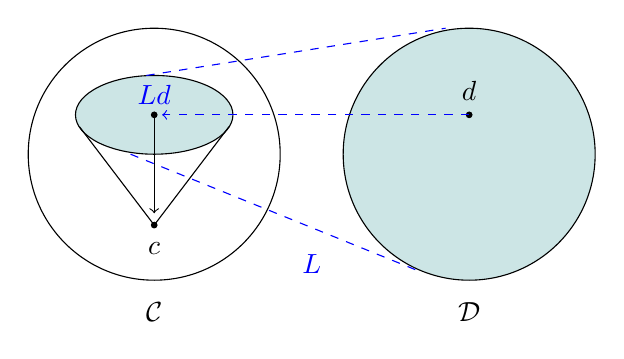
\begin{tikzpicture}
  \def\Xa{2.0};
  \def\Xb{-2.0};
  
  \def\Ytip{-0.9};
  \def\Yo{0.5}; % oval
  \def\Yb{-2.0}; % labels
         \draw (\Xa, 0)[fill=blue!50!green!20]  ellipse (1.6 and 1.6);
         \draw (\Xb , 0) ellipse (1.6 and 1.6);
         % oval
         \draw (\Xb , \Yo)[fill=blue!50!green!20] ellipse (1 and 0.5);
         
        % apex
        \filldraw (\Xb, \Ytip) circle (1pt);
        \node at ( \Xb, \Ytip - 0.3) { $c$ };
        
        % image
        \filldraw (\Xa, \Yo) circle (1pt);
        \node at ( \Xa, \Yo + 0.3) { $d$ };
        
	% middle of the cone
	\draw[->] (\Xb, \Yo) -- (\Xb, \Ytip + 0.15);
        	% sides of the cone
	\draw (\Xb, \Ytip) -- (\Xb + 0.95, \Yo - 0.15);
	\draw (\Xb, \Ytip) -- (\Xb - 0.95, \Yo - 0.15);

        % categories
        \node at (\Xa, \Yb) { $\mathcal D$ };
        \node at (\Xb, \Yb) { $\mathcal C$ };
        \node[blue] at (0, \Yb + 0.6) { $L$ };

        % functor middle
        \filldraw (\Xb, \Yo) circle (1pt);
        \node[blue] at ( \Xb, \Yo + 0.25) { $L d$ };
	\draw[->, blue, dashed] (\Xa, \Yo) -- (\Xb + 0.1, \Yo);
	% functor 
	\draw [blue, dashed] (\Xb - 0.1, \Yo + 0.5    )   --   (\Xa - 0.3, \Yo + 1.1);
	\draw [blue, dashed] (\Xb - 0.3, \Yo - 0.5) -- (\Xa - 0.6, \Ytip - 0.6);
\end{tikzpicture}
\]

The important observation is that this comma category describes a cocone in $\cat C$. The base of this cocone is formed by those objects in the image of $L$ that have an unobstructed view of $c$. The arrows in the base of the cocone are the morphisms in $L/c$. These are exactly the arrows that make the sides of the cocone commute.
\[
 \begin{tikzcd}
 L d
 \arrow[rd, "f"']
 \arrow[rr, "L h"]
 && L d'
 \arrow[ld, "f'"]
 \\
 &c
  \end{tikzcd}
 \hspace{30pt}
\begin{tikzcd}
 d
 \arrow[rr, "h"]
 && d'
  \end{tikzcd}
\]

The base of this cocone can then be projected back to $\cat D$. There is a projection $\pi_c$ which maps every pair $(d, f)$ in  $L/c$ back to $d$, thus forgetting the arrow $f$. It also maps every morphism in $L/c$ to an arrow in $\cat D$ that gave rise to it. This way $\pi_c$ defines a diagram in $\cat D$. The colimit of this diagram exists, because we have assumed that all colimits exist in $\cat D$. Let's call this colimit $t_c$:
\[ t_c = \text{colim}\; \pi_c \]

\[
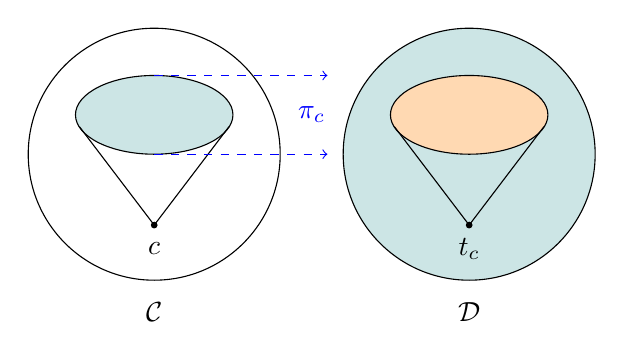
\begin{tikzpicture}
  \def\Xa{2.0};
  \def\Xb{-2.0};
  
  \def\Ytip{-0.9};
  \def\Yo{0.5}; % oval
  \def\Yb{-2.0}; % labels
         \draw (\Xa, 0)[fill=blue!50!green!20]   ellipse (1.6 and 1.6);
         \draw (\Xb , 0) ellipse (1.6 and 1.6);
         % oval
         \draw (\Xb , \Yo)[fill=blue!50!green!20]  ellipse (1 and 0.5);

        % apex
        \filldraw (\Xb, \Ytip) circle (1pt);
        \node at ( \Xb, \Ytip - 0.3) { $c$ };
                
        	% sides of the cone
	\draw (\Xb, \Ytip) -- (\Xb + 0.95, \Yo - 0.15);
	\draw (\Xb, \Ytip) -- (\Xb - 0.95, \Yo - 0.15);

         % second oval
         \draw (\Xa , \Yo) [fill=orange!30]  ellipse (1 and 0.5);
          
        % apex
        \filldraw (\Xa, \Ytip) circle (1pt);
        \node at ( \Xa, \Ytip - 0.3) { $t_c$ };

        	% sides of the cone
	\draw (\Xa, \Ytip) -- (\Xa + 0.95, \Yo - 0.15);
	\draw (\Xa, \Ytip) -- (\Xa - 0.95, \Yo - 0.15);

        % categories
        \node at (\Xa, \Yb) { $\mathcal D$ };
        \node at (\Xb, \Yb) { $\mathcal C$ };
        \node[blue] at (0, \Yo) { $\pi_c$ };

	% functor 
	\draw [->, blue, dashed] (\Xb, \Yo + 0.5) --  (\Xb + 2.2, \Yo + 0.5);
	\draw [->, blue, dashed] (\Xb, \Yo - 0.5)  -- (\Xb + 2.2, \Yo - 0.5);
\end{tikzpicture}
\]

Let's see if we can use this $t_c$ to construct a terminal object in $L/c$. We have to find an arrow, let's call it $\varepsilon_c \colon L t_c \to c$, such that the pair $\langle t_c, \varepsilon_c \rangle$ is terminal in $L/c$. 

Notice that $L$ maps the diagram generated by $\pi_c$ back to the base of the cocone defined by $L/c$. The projection $\pi_c$ did nothing more than to ignore the sides of this cocone, leaving its base intact. 

We now have two cocones in $\cat C$ with the same base: the original one with the apex $c$ and the new one obtained by applying $L$ to the cocone in $\cat D$. Since $L$ preserves colimits, the colimit of the new cocone is $L t_c$---the image of the colimit $t_c$:

\[ \text{colim} \; (L \circ \pi_c) = L ( \text{colim} \; \pi_c) = L t_c\]

By universal construction, we deduce that there must be a unique cocone morphism from the colimit $L t_c$ to $c$. That morphism, which we'll call $\varepsilon_c$, makes all the relevant triangles commute. 

What remains to be shown is that $\langle t_c, \varepsilon_c \rangle$ is terminal in $L/c$, that is, for any  $\langle d, f \colon L d \to c \rangle$ there is a unique comma-category morphism $h \colon d \to t_c$ that makes the following triangle commute:

\[
 \begin{tikzcd}
 L d
 \arrow[rd, "f"']
 \arrow[rr, dashed, "L h"]
 && L t_c
 \arrow[ld, red, "\varepsilon_c"]
 \\
 &c
  \end{tikzcd}
\]

Notice that any such $d$ is automatically part of the diagram produced by $\pi_c$ (it's the result of $\pi_c$ acting on $\langle d, f \rangle$). We know that $t_c$ is the limit of the $\pi_c$ diagram. So there must be a wire from $d$ to $t_c$ in the limiting cocone. We pick this wire as our $h$. 

\[
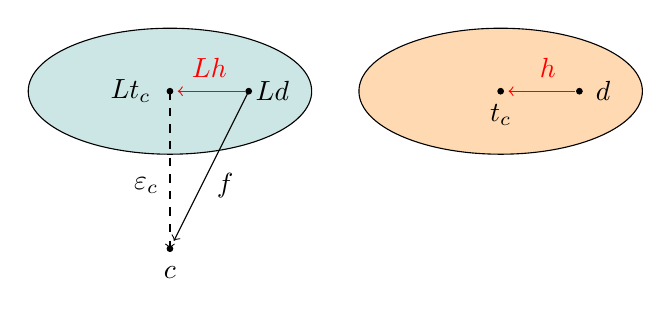
\begin{tikzpicture}
  \def\Xa{2.1};
  \def\Xb{-2.1};
  
  \def\Ytip{0};
  \def\Ybot{-2};
  \def\Yo{0}; % oval
  \def\Yf{-1.2}; % label
         % first oval
         \draw (\Xb , \Yo)[fill=blue!50!green!20]  ellipse (1.8 and 0.8);

         % second oval
         \draw (\Xa , \Yo) [fill=orange!30]  ellipse (1.8 and 0.8);
          
        % apex L tc
        \filldraw (\Xb, \Ytip) circle (1pt);
        \node at ( \Xb - 0.5, \Ytip) { $L t_c$ };
        
        % apex c
        \filldraw (\Xb, \Ybot) circle (1pt);
        \node at ( \Xb, \Ybot - 0.3) { $c$ };
                
        	% sides of the cone L h
	\draw[red, ->]  (\Xb + 0.95, \Yo) -- (\Xb + 0.1, \Ytip);
	\node[red] at (\Xb + 0.5, \Ytip + 0.3) {$L h$};

        % apex tc
        \filldraw (\Xa, \Ytip) circle (1pt);
        \node at ( \Xa, \Ytip - 0.3) { $t_c$ };

        	% sides of the cone h
	\draw [->, red] (\Xa + 0.95, \Yo) -- (\Xa + 0.1, \Ytip);
	\node[red] at ( \Xa + 0.6, \Ytip + 0.3) { $h$ };
	
	% d
        \filldraw (\Xa + 1, \Yo) circle (1pt);
        \node at ( \Xa + 1.3, \Yo) { $d$ };

	% L d
        \filldraw (\Xb + 1, \Yo) circle (1pt);
        \node at ( \Xb + 1.3, \Yo) { $L d$ };
        
        % f
        \draw[->] (\Xb + 1, \Yo) to (\Xb + 0.05, \Ybot + 0.1);
        \node at (\Xb + 0.7, \Yf) {$f$};
        
        % epsilon
        \draw[->, dashed] (\Xb, \Ytip) -- (\Xb, \Ybot);
        \node at (\Xb - 0.3, \Yf) {$\varepsilon_c$};

\end{tikzpicture}
\]
The commuting condition then follows from $\varepsilon_c$ being a morphism between two cocones. It is a unique cocone morphism simply because $\cat D$ is a preorder.

This proves that there is a universal arrow $\langle t_c, \varepsilon_c \rangle$ for every $c$, therefore we have a functor $R$ defined on objects as $R c = t_c$ that is the right adjoint to $L$.

\subsection{Solution set condition}

The problem with the previous proof is that comma categories in most practical cases are large: their objects don't form a set. But maybe we can approximate the comma category by selecting a smaller but representative set of objects and arrows?

To select the objects, we'd use a mapping from some indexing set $I$. We define a set of objects $d_i$ where $i \in I$. Since we are trying to approximate the comma category $L/c$, we select objects together with arrows $f_i \colon L d_i \to c$. 

The relevant part of the comma category is encoded in morphism between objects satisfying the commuting condition. We could try to specialize this condition to only apply inside our family of objects, but that would not be enough. We have to find a way to probe all other objects of the comma category. 

To do this, we reinterpret the commuting condition as a recipe for factorizing an arbitrary $f \colon L d \to c$ through some pair $\langle d_i, f_i \rangle$:
\[
 \begin{tikzcd}
 L d
 \arrow[rd, "f"']
 \arrow[rr, "L h"]
 && \textcolor{red}{L d_i}
 \arrow[ld, red, "f_i"]
 \\
 &c
  \end{tikzcd}
\]

A \index{solution set}\emph{solution set} is a family of pairs $\langle d_i, f_i \colon L d_i \to c \rangle $ indexed by a set $I$ that can be used to factor any pair $\langle d, f \colon L d \to c \rangle $. It means that there exists an index $i \in I$ and an arrow $h \colon d \to d_i$ that factorizes $f$:
\[ f = f_i \circ L h \]

Another way of expressing this property is to say that there exists a \index{weakly terminal set}\emph{weakly terminal} set of object in the comma category $L/c$. A weakly terminal set has the property that for any object in the category there is a morphism to at least one object in the set.

Previously we've seen that having the terminal object in the comma category $L/c$ for every $c$ is enough to define the adjunction. It turns out that we can achieve the same goal using the solution set. 

The assumptions of the Freyd's adjoint functor theorem state that we have a colimit-preserving functor $L \colon \cat D \to \cat C$ from a small co-complete category. Both these conditions relate to \emph{small} diagrams. If we can pick a solution set $\langle d_i, f_i \colon L d_i \to c \rangle $ for every $c$, then the right adjoint $R$ exists. Solution sets for different $c$'s may be different.

We've seen before that in a cocomplete category the existence of a weakly terminal set is enough to define a terminal object. In our case it means that, for any $c$, we can construct the universal arrow from $L$ to $c$. And this is enough to define the whole adjunction.

A dual version of the adjoint functor theorem can be used to construct the left adjoint.

\subsection{Defunctionalization}

Every programming language lets us define functions, but not all languages support higher level functions (functions taking functions as arguments, functions returning functions, or data types constructed from functions) or anonymous functions (a.k.a., lambdas). It turns out that, even in such languages, higher order functions can be implemented using the process called defunctionalization. This technique is based on the adjoint functor theorem. Moreover, defunctionalization can be used whenever passing functions around is impractical, for instance in a distributed system.

The idea behind defunctionalization is that the function type is defined as the right adjoint to the product. 
\[ \cat C(e \times a, b) \cong \cat C(e, b^a) \]
The adjoint functor theorem can be used to approximate this adjoint. 

In general, any finite program can only have a finite number of function definitions. These functions (together with the environments they capture) form the solution set that we can use to construct the function type. In practice, we do it only for a small subset of functions which occur as arguments to, or are returned from, other functions.

A typical example of the usage of higher order functions is in continuation passing style. For instance, here's a function that calculates the sum of the elements of a list. But instead of returning the sum it calls a continuation \hask{k} with the result:
\begin{haskell}
sumK :: [Int] -> (Int -> r) -> r
sumK [] k = k 0
sumK (i : is) k =
  sumK is (\s -> k (i + s))
\end{haskell}
If the list is empty, the function calls the continuation with zero. Otherwise it calls itself recursively, with two arguments: the tail of the list \hask{is}, and a new continuation:
\begin{haskell}
\s -> k (i + s)
\end{haskell}
This new continuation calls the previous continuation \hask{k}, passing it the sum of the head of the list and its argument \hask{s} (which is the accumulated sum). 

Notice that this lambda is a closure: It's a function of one variable \hask{s}, but it also has access to \hask{k} and \hask{i} from its environment.

To extract the final sum, we call our recursive function with the trivial continuation, the identity:
\begin{haskell}
sumList :: [Int] -> Int
sumList as = sumK as (\i -> i)
\end{haskell}

Anonymous functions are convenient, but nothing prevents us from using named functions. However, if we want to factor out the continuations, we have to be explicit about passing in the environments. 

For instance, we can replace our first lambda:
\begin{haskell}
\s -> k (i + s)
\end{haskell}
with the function \hask{more}, but we have to explicitly pass the pair \hask{(i, k)} as the environment of the type \hask{(Int, Int -> r)}:
\begin{haskell}
more :: (Int, Int -> r) -> Int -> r
more (i, k) s = k (i + s)
\end{haskell}
The other lambda, the identity, uses the empty environment, so it becomes:
\begin{haskell}
done :: Int -> Int
done i = i
\end{haskell}
Here's the implementation of our algorithm using these two named functions:
\begin{haskell}
sumK' :: [Int] -> (Int -> r) -> r
sumK' [] k = k 0
sumK' (i : is) k =
  sumK' is (more (i, k))
\end{haskell}

\begin{haskell}
sumList :: [Int] -> Int
sumList is = sumK' is done
\end{haskell}

In fact, if all we are interested in is calculating the sum, we can replace the polymorphic type \hask{r} with \hask{Int} with no other changes.

This implementation still uses higher order functions. In order to eliminate them, we have to analyze what it means to pass a function as an argument. Such a function can only be used in one way: it can be applied to its arguments. This property of a function type is expressed as the counit of the currying adjunction:
\[ \varepsilon \colon b^a \times a \to b \]
or, in Haskell, as a higher-order function:
\begin{haskell}
apply :: (a -> b, a) -> b
\end{haskell}
This time we are interested in constructing the counit from first principles. We've seen that this can be accomplished using the comma category. In our case, an object of the comma category for the product functor $L_a = (-) \times a$ is a pair 
\[(e, f \colon (e \times a) \to b) \]
or, in Haskell:
\begin{haskell}
data Comma a b e = Comma e ((e, a) -> b)
\end{haskell}
A morphism in this category between $(e, f)$ and $(e', f')$ is an arrow $h \colon e \to e'$, which satisfies the commuting condition:
\[ f' \circ h = f \]
We interpret this morphism as ``reducing'' the environment $e$ down to $e'$. The arrow $f'$ is able to produce the same output of the type $b$ using a potentially smaller environment given by $h (e)$. For instance $e$ may contain variables that are irrelevant for computing $b$ from $a$, and $h$ projects them out. 

\[
 \begin{tikzcd}
 e \times a
 \arrow[rd, "f"']
 \arrow[rr, "h \times a"]
 && e' \times a
 \arrow[ld, "f'"]
 \\
 &b
  \end{tikzcd}
 \hspace{30pt}
\begin{tikzcd}
 e
 \arrow[rr, "h"]
 && e'
  \end{tikzcd}
\]


In fact, we performed this kind of reduction when defining \hask{more} and \hask{done}. In principle, we could have passed the tail \hask{is} to both functions, since it's accessible at the point of call. But we knew that they didn't need it.

Using the Freyd's theorem, we could define the function object $a \to b$ as the colimit of the diagram defined by the comma category. Such a colimit is essentially a giant coproduct of all environments modulo identifications given by comma-category morphisms. These identification do the job of reducing the environment needed by $a \to b$ to the bare minimum. 

In our example, the continuations we're interested in are functions \hask{Int -> Int}. In fact we are not interested in generating the generic function type \hask{Int -> Int}; just the minimal one that would accommodate our two functions \hask{more} and \hask{done}. We can do it by creating a very small solution set. 

In our case the solution set consists of pairs $(e_i, f_i \colon e_i \times a \to b)$ such that any pair $(e, f \colon e \times a \to b)$ can be factorized through one of the $f_i$'s. More precisely, the only two environments we're interested in are \hask{(Int, Int ->Int)} for \hask{more}, and the empty environment \hask{()} for \hask{done}. 

In principle, our solution set should allow for the factorization of every object of the comma category, that is a pair of the type:
\begin{haskell}
(e, (e, Int) -> Int)
\end{haskell}
but here we are only interested in two specific functions. Also, we are not concerned with the uniqueness of the representation so, instead of using a colimit (as we did for the adjoint functor theorem), we'll just use a coproduct of all the environments of interest. We end up with the following data type that is the sum of the two environments, \hask{()} and \hask{(Int, Int -> Int)}, we're interested in. We end up with the type:
\begin{haskell}
data Kont = Done | More Int Kont
\end{haskell}
Notice that we have recursively encoded the \hask{Int->Int} part of the environment as \hask{Kont}. Thus we have also removed the need to use functions as arguments to data constructors.

If you look at this definition carefully, you will discover that it's the definition of a list of \hask{Int}, modulo some renamings. Every call to \hask{More} pushes another integer on the \hask{Kont} stack. This interpretation agrees with our intuition that recursive algorithms require some kind of a runtime stack. 

We are now ready to implement our approximation to the counit of the adjunction. It's composed from the bodies of the two functions, with the understanding that recursive calls also go through \hask{apply}:
\begin{haskell}
apply :: (Kont, Int) -> Int
apply (Done, i) = i
apply (More i k, s) = apply (k, i + s)
\end{haskell}
Compare this with our earlier:
\begin{haskell}
done i = i
more (i, k) s = k (i + s)
\end{haskell}


The main algorithm can now be rewritten without any higher order functions or lambdas:
\begin{haskell}
sumK'' :: [Int] -> Kont -> Int
sumK'' [] k = apply (k, 0)
sumK'' (i : is) k = sumK'' is (More i k)
\end{haskell}

\begin{haskell}
sumList'' is = sumK'' is Done
\end{haskell}

The main advantage of defunctionalization is that it can be used in distributed environments. Arguments to remote functions, as long as they are data structures and not functions, can be serialized and send along the wire. All that's needed is for the receiver is have access to \hask{apply}. 

\section{Free/Forgetful Adjunctions}
The two functors in the adjunction play different roles: the picture of the adjunction is not symmetric. Nowhere is this illustrated better than in the case of the free/forgetful adjunctions. 

A forgetful functor is a functor that ``forgets'' some of the structure of its source category. This is not a rigorous definition but, in most cases, it's pretty obvious what structure is being forgotten. Very often the target category is just the category of sets, which is considered the epitome of structurelessness. The result of the forgetful functor in that case is called the ``underlying'' set, and the functor itself is often called $U$. 

More precisely, we say that a functor forgets \emph{structure} if the mapping of hom-sets is not surjective, that is, there are arrows in the target hom-set that have no corresponding arrows in the source hom-set. Intuitively, it means that the arrows in the source have some structure to preserve, so there are fewer of them; and that structure is absent in the target. 

The left adjoint to a forgetful functor is called a \emph{free functor}.

\[
 \begin{tikzcd}
F x
\arrow[d, bend right, red, dashed]
\arrow[d, dashed]
\arrow[d, bend left, blue, dashed]
  &&
  x
\arrow[d, bend right, red, dashed]
\arrow[d, dashed]
\arrow[d, bend left, blue, dashed]
 \arrow[ll, bend right, "F"']
 \\
y
   \arrow[rr, bend right, "U"']
 &&
 U y
  \end{tikzcd}
\]

A classic example of a free/forgetful adjunction is the construction of the free monoid.


\subsection{The category of monoids}
Monoids in a monoidal category $\mathcal{C}$ form their own category $\mathbf{Mon}(\mathcal{C})$. Its objects are monoids, and its arrows are the arrows of $\mathcal{C}$ that preserve the monoidal structure. 

The following diagram explains what it means for $f$ to be a monoid morphism, going from a monoid $(M_1, \eta_1, \mu_1)$ to a monoid $(M_2, \eta_2, \mu_2)$:
\[
 \begin{tikzcd}
 & M_1
 \arrow[dd, "f"]
 & M_1 \otimes M_1
 \arrow[l, "\mu_1"]
 \arrow[dd, "f \otimes f"]
 \\
 I
 \arrow[ru, "\eta_1"]
 \arrow[rd, "\eta_2"']
 \\
 & M_2
 & M_2 \otimes M_2
 \arrow[l, "\mu_2"]
  \end{tikzcd}
\]
A monoid morphism $f$ must map unit to unit, which means that:
\[ f \circ \eta_1 = \eta_2 \]
and it must map multiplication to multiplication:
\[ f \circ \mu_1 = \mu_2 \circ (f \otimes f)\]
Remember, the tensor product $\otimes$ is functorial, so it can lift pairs of arrows, as in $f \otimes f$.

In particular, the category $\mathbf{Set}$ is monoidal, with cartesian product and the terminal object providing the monoidal structure. 

In particular, monoids in $\mathbf{Set}$ are sets with additional structure. They form their own category $\mathbf{Mon}(\mathbf{Set})$ and there is a forgetful functor $U$ that simply maps the monoid to the set of its elements. When we say that a monoid is a set, we mean the underlying set.

\subsection{Free monoid}

We want to construct the free functor 
\[ F \colon \mathbf{Set} \to \mathbf{Mon}(\mathbf{Set})\]
that is adjoint to the forgetful functor $U$. 

We start with an arbitrary set $X$ and an arbitrary monoid $m$. On the right-hand side of the adjunction we have the set of functions from $X$ to $U m$. On the left-hand side, we have a set of highly constrained structure-preserving monoid morphisms from $F X$ to $m$. How can these two hom-sets be isomorphic?

In  $\mathbf{Mon}(\mathbf{Set})$, monoids are sets of elements, and monoid morphisms are functions between such sets, satisfying additional constraints: preserving unit and multiplication. 

Arrows in $\mathbf{Set}$, on the other hand, are just functions with no additional constraints. So, in general, there are fewer arrows between monoids than there are between their underlying sets. 

\[
 \begin{tikzcd}
F X
\arrow[d, bend right, red, dashed]
\arrow[d, dashed]
\arrow[d, bend left, blue, dashed]
  &&
X
\arrow[d, bend right, red, dashed]
\arrow[d, dashed]
\arrow[d, bend left, blue, dashed]
 \arrow[ll, bend right, "F"']
 \\
m
   \arrow[rr, bend right, "U"']
 &&
 U m
  \end{tikzcd}
\]

Here's the idea: if we want to have a one to one matching between arrows, we want $F X$ to be much larger than $X$. This way, there will be many more functions from it to $m$---so many that, even after rejecting the ones that don't preserve the structure, we'll still have enough to match every function $f \colon X \to U m$.

We'll construct the monoid $F X$ starting from the set $X$, and adding more and more elements as we go. We'll call the initial set $X$ the \index{generators of a monoid}\emph{generators} of $F X$. We'll construct a monoid morphism $g \colon F X \to m$ starting with the original function $f$ and extending it to act on more and more elements.

On generators, $x \in X$, $g$ works the same as $f$:
\[ g x = f x \]

Since $F X$ is supposed to be a monoid, it has to have a unit. We can't pick one of the generators to be the unit, because it would impose constraints on the part of $g$ that is already fixed by $f$---it would have to map it to the unit $e'$ of $m$. So we'll just add an extra element $e$ to $F X$ and call it the unit. We'll define the action of $g$ on it by saying that it is mapped to the unit $e'$ of $m$:
\[ g e = e' \]

We also have to define monoidal multiplication in $F X$. Let's start with a product of two generators $a$ and $b$. The result of the multiplication cannot be another generator because, again, that would constrain the part of $g$ that's fixed by $f$---products must be mapped to products. So we have to make all products of generators new elements of $F X$. Again, the action of $g$ on those products is fixed:
\[ g (a \cdot b)  = g a \cdot g b\]

Continuing with this construction, any new multiplication produces a new element of $F X$, except when it can be reduced to an existing element by applying monoid laws. For instance, the new unit $e$ times a generator $a$ must be equal to $a$. But we have made sure that $e$ is mapped to the unit of $m$, so the product $g e \cdot g a$ is automatically equal to $g a$.

Another way of looking at this construction is to think of the set $X$ as an alphabet. The elements of $F X$ are then strings of characters from this alphabet. The generators are single-letter strings, ``$a$'', ``$b$'', and so on. The unit is an empty string ``''. Multiplication is string concatenation, so  ``$a$'' times ``$b$'' is a new string ``$ab$''. Concatenation is automatically associative and unital, with the empty string as the unit.

The intuition behind free functors is that they generate structure ``freely,'' as in ``with no additional constraints.'' They also do it lazily: instead of performing operations, they just record them. They create generic domain-specific programs that can be executed later by specific interpreters.

The free monoid ``remembers to do the multiplication'' at a later time. It stores the arguments to multiplication in a string, but doesn't perform the multiplication. It's only allowed to simplify its records based on generic monoidal laws. For instance, it doesn't have to store the command to multiply by the unit. It can also ``skip the parentheses'' because of associativity. 

\begin{exercise}
What is the unit and the counit of the free monoid adjunction $F \dashv U$?
\end{exercise}

\subsection{Free monoid in programming}

In Haskell, monoids are defined using the following typeclass:
\begin{haskell}
class Monoid m where
  mappend :: m -> m -> m
  mempty  :: m
\end{haskell}
Here, \hask{mappend} is the curried form of the mapping from the product: \hask{(m, m) -> m}. The \hask{mempty} element corresponds to the arrow from the terminal object (unit of the monoidal category), or simply an element of \hask{m}. 

A free monoid generated by some type \hask{a}, which serves as a set of generators, is represented by a list type \hask{[a]}. An empty list serves as the unit; and monoid multiplication is implemented as list concatenation, traditionally written in infix form:
\begin{haskell}
(++) :: [a] -> [a] -> [a]
(++) []     ys = ys
(++) (x:xs) ys = x : xs ++ ys
\end{haskell}
A list is an instance of a \hask{Monoid}:
\begin{haskell}
instance Monoid [a] where
  mempty = []
  mappend = (++)
\end{haskell}

To show that it's a free monoid, we have to be able to construct a monoid morphism from the list of \hask{a} to an arbitrary monoid \hask{m}, provided we have an (unconstrained) mapping from \hask{a} to (the underlying set of) \hask{m}. We can't express all of this in Haskell, but we can define the function:
\begin{haskell}
foldMap :: Monoid m => (a -> m) -> ([a] -> m)
foldMap f = foldr mappend mempty . fmap f
\end{haskell}
This function transforms the elements of the list to monoidal values using \hask{f} and then folds them using \hask{mappend}, starting with the unit \hask{mempty}. 

It's easy to see that an empty list is mapped to the monoidal unit. It's not too hard to see that a concatenation of two lists is mapped to the monoidal product of the results. So, indeed, \hask{foldMap} is a monoid morphism. 

Following the intuition of a free monoid being a domain-specific program for multiplying stuff, \hask{foldMap} provides an \emph{interpreter} for this program. It performs all the multiplications that have been postponed. Note that the same program may be interpreted in many different ways, depending on the choice of the concrete monoid and the function \hask{f}.

We'll come back to free monoids as lists in the chapter on algebras.

\begin{exercise}
Write a program that takes a list of integers and interprets it in two different ways: once using the additive and once using the multiplicative monoid of integers.
\end{exercise}

\section{The Category of Adjunctions}
We can define composition of adjunctions by taking advantage of the composition of functors that define them. Two adjunctions, $L \dashv R$ and $L' \dashv R'$, are composable if they share the category in the middle:
\[
 \begin{tikzcd}
  \mathcal{C}
  \arrow[rr, bend right, "R'"']
  &&
  \mathcal{D}
  \arrow[ll, bend right, "L'"']
    \arrow[rr, bend right, "R"']
&&
  \mathcal{E}
  \arrow[ll, bend right, "L"']
 \end{tikzcd}
\]
By composing the functors we get a new adjunction $(L' \circ L) \dashv (R \circ R')$. 

Indeed, let's consider the hom-set:
\[ \mathcal{C}(L' (L e), c) \]
Using the $L' \dashv R'$ adjunction, we can transpose $L'$ to the right, where it becomes $R'$:
\[ \mathcal{D}(L e, R' c) \]
and using $L \dashv R$ we can similarly transpose $L$:
\[ \mathcal{E}( e, R(R' c)) \]
Combining these two isomorphisms, we get the composite adjunction:
\[ \mathcal{C}((L' \circ L) e, c) \cong \mathcal{E}( e, (R \circ R') c)\]

Because functor composition is associative, the composition of adjunctions is also associative. It's easy to see that a pair of identity functors forms a trivial adjunction that serves as the identity with respect to composition of adjunctions. Therefore we can define a category $\mathbf{Adj}(\mathbf{Cat})$ in which objects are categories and arrows are adjunctions (by convention, pointing in the direction of the left adjoint). 

Adjunctions can be defined purely in terms of functors and natural transformations, that is 1-cells and 2-cells in the 2-category $\mathbf{Cat}$. There is nothing special about $\mathbf{Cat}$, and in fact adjunctions can be defined in any 2-category. Moreover, the category of adjunctions is itself a 2-category.

\section{Levels of Abstraction}

Category theory is about structuring our knowledge. In particular, it can be applied to the knowledge of category theory itself. Hence we see a lot of mixing of abstraction levels in category theory. The structures that we see at one level can be grouped into higher-level structures which exhibit even higher levels of structure, and so on. 

In programming we are used to building hierarchies of abstractions. Values are grouped into types, types into kinds. Functions that operate on values are treated differently than functions that operate on types. We often use different syntax to separate levels of abstractions. Not so in category theory.

A set, categorically speaking, can be described as a discrete category. Elements of the set are objects of this category and, other than the obligatory identity morphisms, there are no arrows between them. 

The same set can then be seen as an object in the category $\mathbf{Set}$. Arrows in this category are functions between sets.

The category $\mathbf{Set}$, in turn, is an object in the category $\mathbf{Cat}$. Arrows in $\mathbf{Cat}$ are functors. 

Functors between any two categories $\mathcal{C}$ and $\mathcal{D}$ are objects in the functor category $[\mathcal{C}, \mathcal{D}]$. Arrows in this category are natural transformations.

We can define functors between functor categories, product categories, opposite categories, and so on, ad infinitum. 

Completing the circle, hom-sets in every category are sets. We can define mappings and isomorphisms between them, reaching across disparate categories. Adjunctions are possible because we can compare hom-sets that live in different categories.

\end{document}